\documentclass[12pt]{article}
 
\usepackage[margin=1in]{geometry} 
\usepackage{amsmath,amsthm,amssymb}
\usepackage{graphicx}
\usepackage{paralist}
 
\newenvironment{theorem}[2][Theorem]{\begin{trivlist}
\item[\hskip \labelsep {\bfseries #1}\hskip \labelsep {\bfseries #2.}]}{\end{trivlist}}

\newenvironment{postulate}[1][Postulate]{\begin{trivlist}
\item[\hskip \labelsep {\bfseries #1}]}{\end{trivlist}}

\begin{document}
 
% --------------------------------------------------------------
%                         Start here
% --------------------------------------------------------------
 
\title{Relocating a Segment} 
\author{Theron J Hitchman}  
\maketitle

{%
\centering
\textit{Communicated by: Dr. Hitchman}
\par
}
\hrule
\vspace{.2in}


This is our second example paper, and the second reworking of an argument in Euclid's \emph{Elements} into more modern language. Our choice this week is a construction proposition, which helps us to move a segment to another location.

Our argument will rely on an important fact that Euclid uses but does not state explicitly. Since the fact is pretty easy to just accept as obvious, the easiest thing for us to do at this point is to add the following to our list of assumptions. 

\begin{postulate}[Circle-Ray Intersection Property] Suppose that $\mathcal{C}$ is a circle and that $r$ is a ray with initial point $X$. If there is a point $Y$ which lies on $r$, is in the interior of $C$, and is distinct from $X$, then $\mathcal{C}$ and $r$ intersect at a point $Z$ so that $Y$ lies between $X$ and $Z$ on $r$.
\end{postulate}

\begin{figure}[ht]
\centering
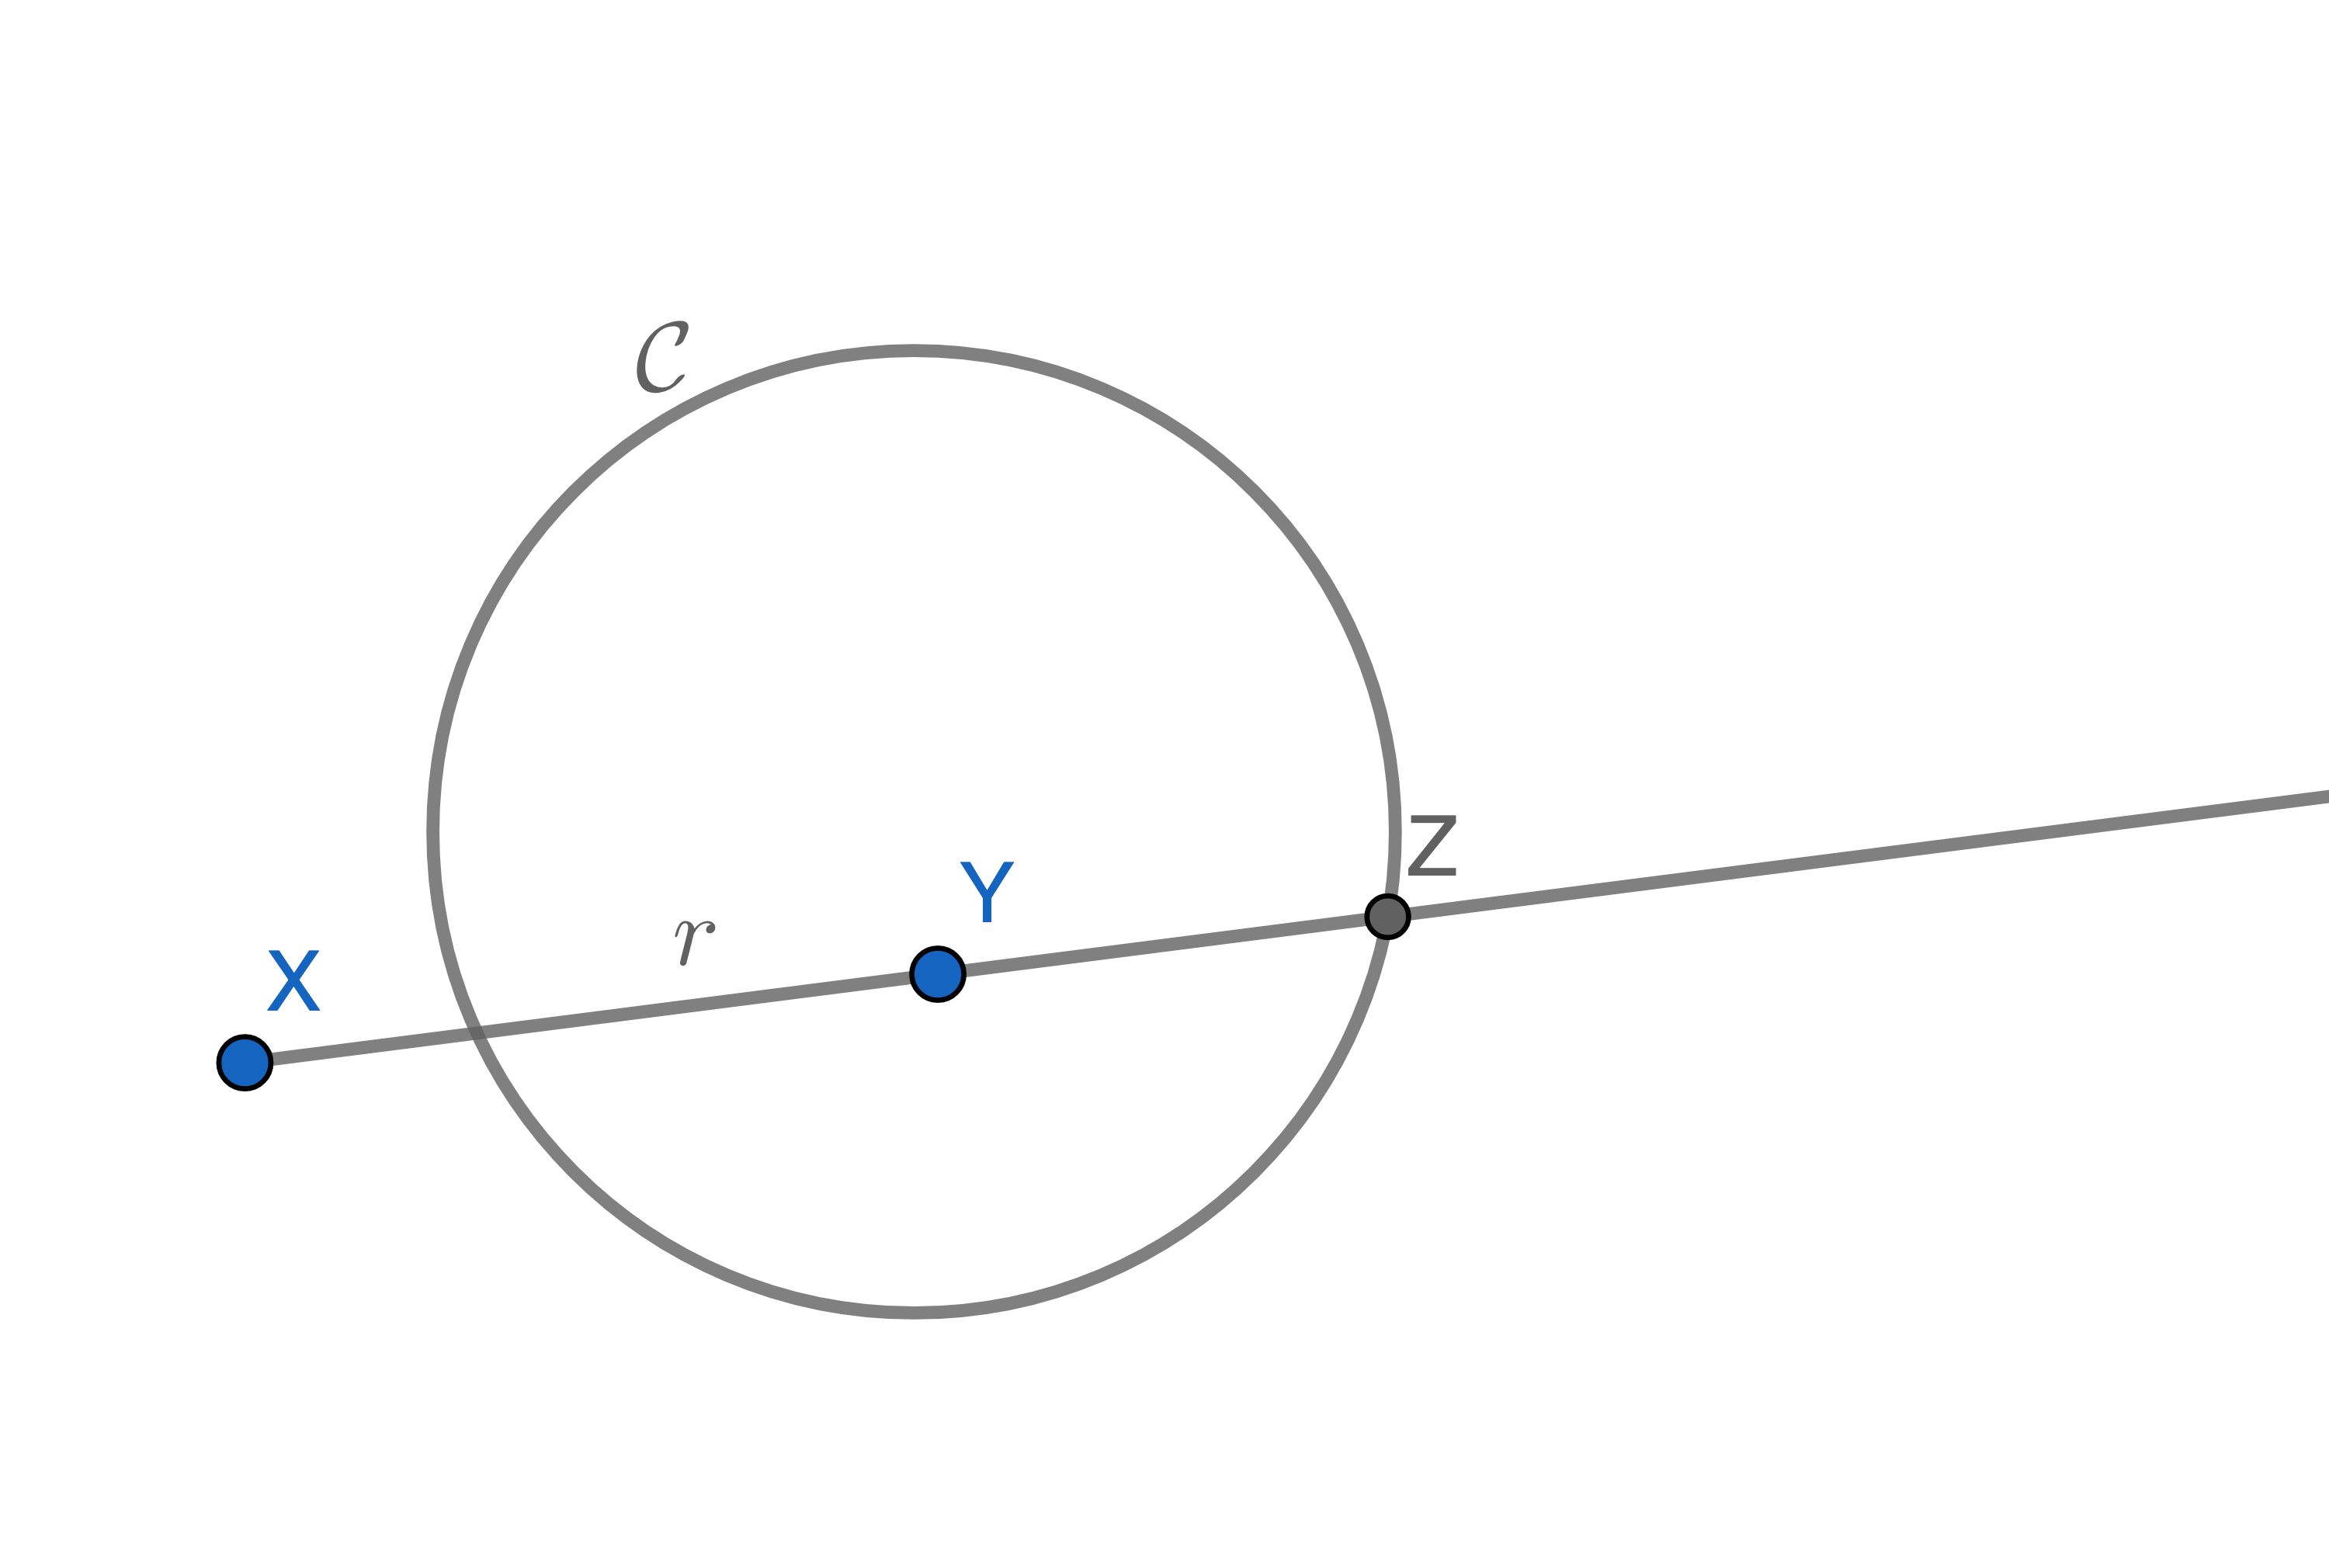
\includegraphics[width=.35\textwidth]{example2-postulate.png}
\caption{Circle-Ray Intersection Property}
\end{figure}

It is a difficult challenge to write down a set of postulates which is complete enough to do all of the interesting geometry, but is not too large to keep track of everything. Euclid's attempt is a good one, but there are several tricky, technical things like this that he missed. You should note that this is a lot like the Circle-Circle Intersection Property required to get Proposition I.1 to work.

Now, with this property in our pocket, we are ready to get to our main goal.
\clearpage

\begin{theorem}{I.2}[Euclid's Proposition 2 from Book I of \emph{The Elements}]
Let $AB$ be a given segment, and let $X$ be a point. Then it is possible to construct, with a straightedge and compass, a segment $XY$ which is congruent to $AB$.
\end{theorem}
 
\begin{proof}
We shall first describe the construction process, and then argue for why it works. 
\begin{compactenum}
\item Construct an equilateral triangle which has $AX$ as one side.
	\begin{compactenum}
	\item Draw a circle with center $A$ passing through $X$.
	\item Draw a circle with center $X$ passing through $A$. Choose a point $C$ where these two circles meet.
	\item Draw segments $XA$, $AC$ and $CX$.
	\end{compactenum}
\item Extend segment $CA$ to a ray starting at $C$ which passes through $C$.
\item Draw the circle with center $A$ which passes through $B$. Where the ray $CA$ meets this circle, we find a new point $D$.
\item Extend the segment $CX$ to a ray starting at $C$ which passes through $X$.
\item Draw the circle with center $C$ which passes through $D$. Where the ray $XC$ meets this circle, we find a new point $Y$
\end{compactenum}

\begin{figure}[ht]
\centering
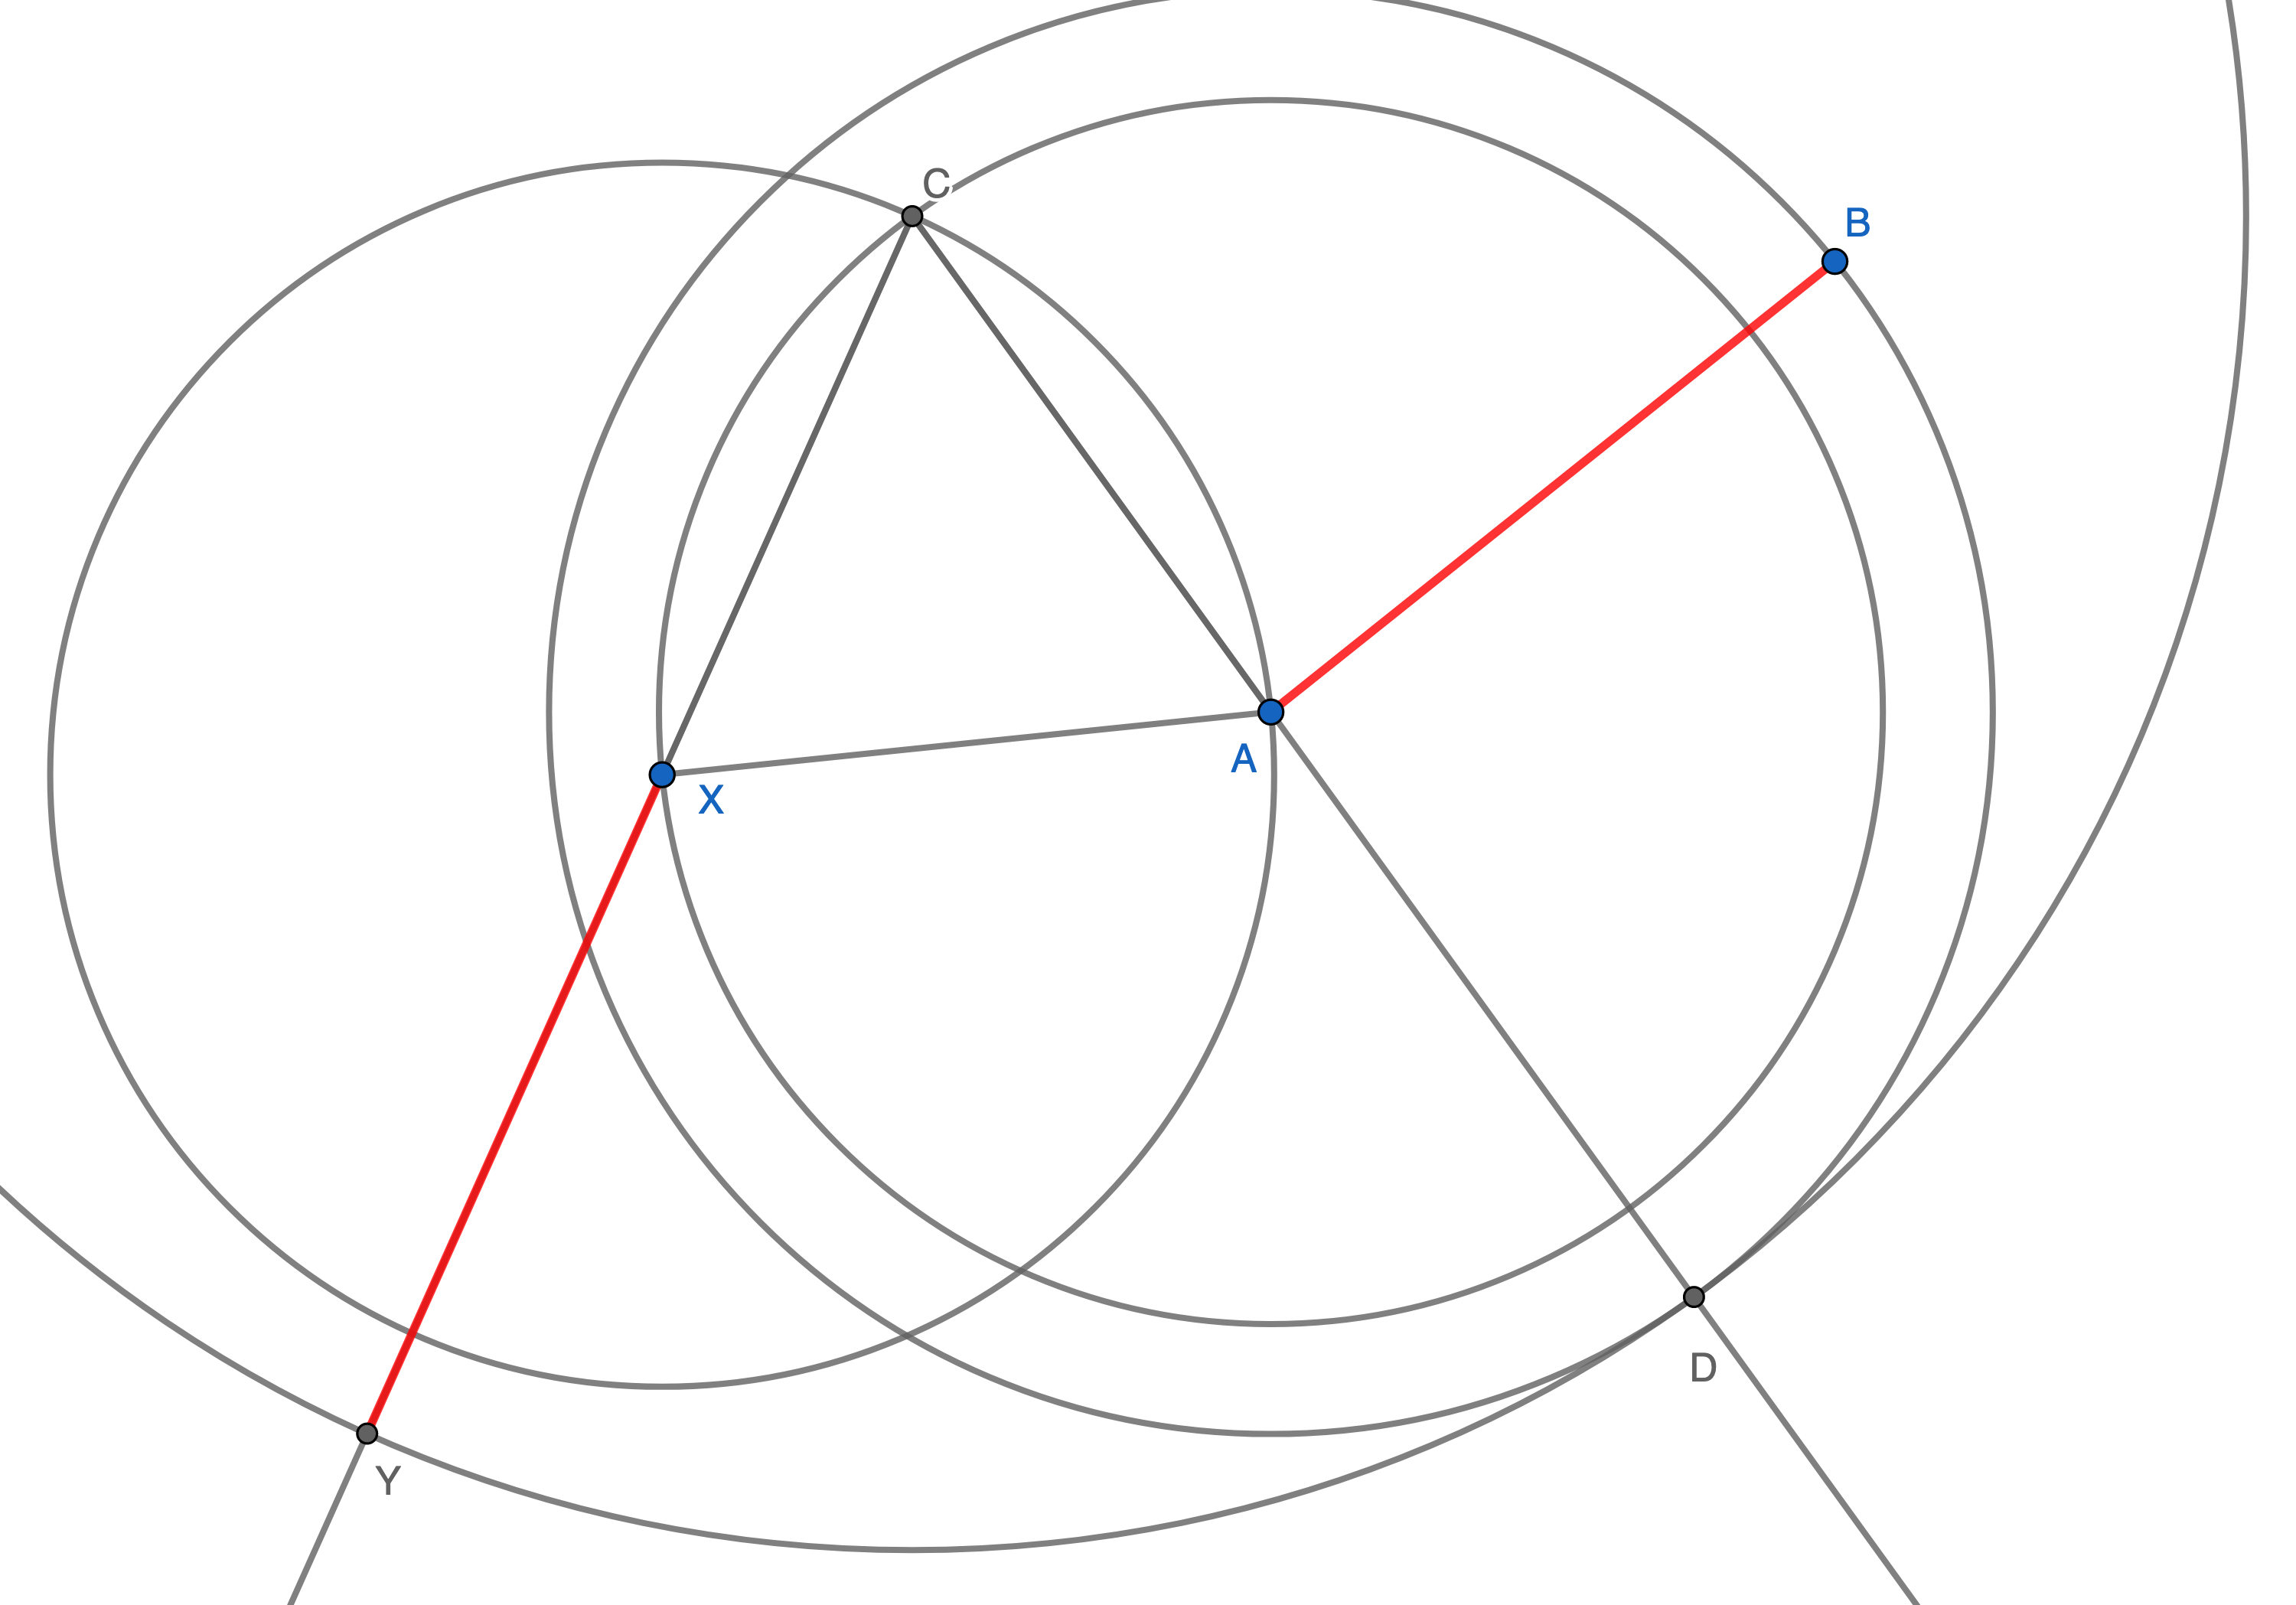
\includegraphics[width=.65\textwidth]{example2-img.png}
\caption{The construction}
\end{figure}

We claim that this construction is possible as described, and that the segment $XY$ is congruent to the segment $AB$. 

To see that this construction is possible, first note that nearly all of the steps are to (1) draw a segment given two points, (2) extend a segment to a ray, or (3) draw a circle given the center and a point which should lie on the circumference. These steps are all justified by Euclid's first three postulates, in that order. That is, we can draw a segment using Euclid's Postulate 1, extend a segment using Euclid's Postulate 2, and draw a circle using Euclid's Postulate 3. The steps that need more consideration are those asserting that we can find a new point by looking for the intersection of two objects. But those are justified by an appeal to the Circle-Ray Intersection Property.

Next, we must show that the segments $AB$ and $XY$ are congruent. Our argument is mostly a repeated use of the definition of a circle, which is defintion 15 in Book I of Euclid's \emph{Elements}
First, note that since $AB$ and $AD$ are radii of the circle $\odot AB$, they must be congruent by the definition of a circle. Similarly, the segments $CD$ and $CY$ are congruent since they are both radii of the circle $\odot CD$.

Also, since the first step of our construction is to create the equilateral triangle $CAX$. This is exactly the work in Euclid's Proposition I.1, and we deduce that $CA$ is congruent to $CX$. Now, the congruent segments $CY$ and $CD$ contain the congruent segments $CX$ and $CA$, so by Euclid's Common Notion 3, we deduce that $XY$ is congruent to $AD$. Recall that $AD$ is also congruent to $AB$, hence by Euclid's Common Notion 1, the segments $XY$ and $AB$ are congruent.

Therefore, segment $XY$ is the segment we are required to construct, and the proof is complete.
\end{proof}

\vspace{1in}

\hrule

\begin{center}
A Comment
\end{center}

\hrule

\vspace{0.25in}

This paper is rather longer than Euclid's version of the same argument. The first reason for this is that we were more careful about the Circle-Ray Intersection Property, and that took some space to describe. The second reason is that we have been very careful to explain every single step, including the use of Postulates, Common Notions and the definition of a circle. This choice is driven by the fact that we are still beginners. As time goes on these low-to-the ground deductions will become tiresome (you will begin to find them ``obvious''), and we will stop making them explicit. More experience will give you a sense of which steps can be done without saying, and which steps need to be written out.
 
\end{document}